\documentclass[landscape,a0paper,fontscale=0.292]{baposter}

\usepackage[vlined]{algorithm2e}
\usepackage{times}
\usepackage{calc}
\usepackage{url}
\usepackage{graphicx}
\usepackage{amsmath}
\usepackage{amssymb}
\usepackage{relsize}
\usepackage{multirow}
\usepackage{booktabs}

\usepackage{graphicx}
\usepackage{multicol}
\usepackage[T1]{fontenc}
\usepackage{ae}
\usepackage{enumitem}

\usepackage{colortbl}
\usepackage{xcolor}
\graphicspath{{images/}}

\setlist[itemize]{leftmargin=*,nosep}
 \setlength{\columnsep}{0.7em}
 \setlength{\columnseprule}{0mm}


% %%%%%%%%%%%%%%%%%%%%%%%%%%%%%%%%%%%%%%%%%%%%%%%%%%%%%%%%%%%%%%%%%%%%%%%%%%%%%%%%
% % Save space in lists. Use this after the opening of the list
% %%%%%%%%%%%%%%%%%%%%%%%%%%%%%%%%%%%%%%%%%%%%%%%%%%%%%%%%%%%%%%%%%%%%%%%%%%%%%%%%
 \newcommand{\compresslist}{%
 \setlength{\itemsep}{0pt}%
 \setlength{\parskip}{0pt}%
 \setlength{\parsep}{0pt}%
 }
\renewcommand{\rmdefault}{ptm} % Arial
\renewcommand{\sfdefault}{ptm} % Arial

%%%%%%%%%%%%%%%%%%%%%%%%%%%%%%%%%%%%%%%%%%%%%%%%%%%%%%%%%%%%%%%%%%%%%%%%%%%%%
%% Begin of Document
%%%%%%%%%%%%%%%%%%%%%%%%%%%%%%%%%%%%%%%%%%%%%%%%%%%%%%%%%%%%%%%%%%%%%%%%%%%%%
\begin{document}
%%%%%%%%%%%%%%%%%%%%%%%%%%%%%%%%%%%%%%%%%%%%%%%%%%%%%%%%%%%%%%%%%%%%%%%%%%%%%
%% Here starts the poster
%%---------------------------------------------------------------------------
%% Format it to your taste with the options
%%%%%%%%%%%%%%%%%%%%%%%%%%%%%%%%%%%%%%%%%%%%%%%%%%%%%%%%%%%%%%%%%%%%%%%%%%%%%
\begin{poster}{
 % Show grid to help with alignment
 grid=false,
 columns=4,
 % Column spacing
 colspacing=0.7em,
 % Color style
 headerColorOne=cyan!20!white!90!black,
 borderColor=cyan!30!white!90!black,
 % Format of textbox
 textborder=faded,
 % Format of text header
 headerborder=open,
 headershape=roundedright,
 headershade=plain,
 background=none,
 bgColorOne=cyan!10!white,
 headerheight=0.12\textheight}
 % Eye Catcher
 {
      
\includegraphics[width=0.08\linewidth]{HKU_logo}
      \makebox[0.04\textwidth]{} 
 }
 % Title
 {\sc\huge\bf TOM-Net: Learning Transparent Object Matting from a Single Image}
 % Authors
 {\vspace{0.3em} Guanying Chen*, Kai Han*, Kwan-Yee K. Wong \\[0.2em]
 {The University of Hong Kong \\[0.2em] (* indicates equal contribution)}}
 %{\texttt{\{gychen, khan, kykwong\}@cs.hku.hk}}}
 % University logo
 {
  \begin{tabular}{r}
      %\makebox[0.01\textwidth]{} 
    
\includegraphics[width=0.12\linewidth]{cvpr18logo_3.jpg}
  \end{tabular}
 }

%%%%%%%%%%%%%%%%%%%%%%%%%%%%%%%%%%%%%%%%%%%%%%%%%%%%%%%%%%%%%%%%%%%%%%%%%%%%%%
%%% Now define the boxes that make up the poster
%%%---------------------------------------------------------------------------
%%% Each box has a name and can be placed absolutely or relatively.
%%% The only inconvenience is that you can only specify a relative position 
%%% towards an already declared box. So if you have a box attached to the 
%%% bottom, one to the top and a third one which should be inbetween, you 
%%% have to specify the top and bottom boxes before you specify the middle 
%%% box.
%%%%%%%%%%%%%%%%%%%%%%%%%%%%%%%%%%%%%%%%%%%%%%%%%%%%%%%%%%%%%%%%%%%%%%%%%%%%%%

%%%%%%%%%%%%%%%%%%%%%%%%%%%%%%%%%%%%%%%%%%%%%%%%%%%%%%%%%%%%%%%%%%%%%%%%%%%%%%
\headerbox{\bf\color{blue} Problem Definition and Contribution}{name=contribution,column=0,row=0,span=1}{
   \textbf{\color{blue}Goal:} Image matting for colorless transparent object from a single image.
    \begin{center}
        \vspace{-0.8em}
        \centering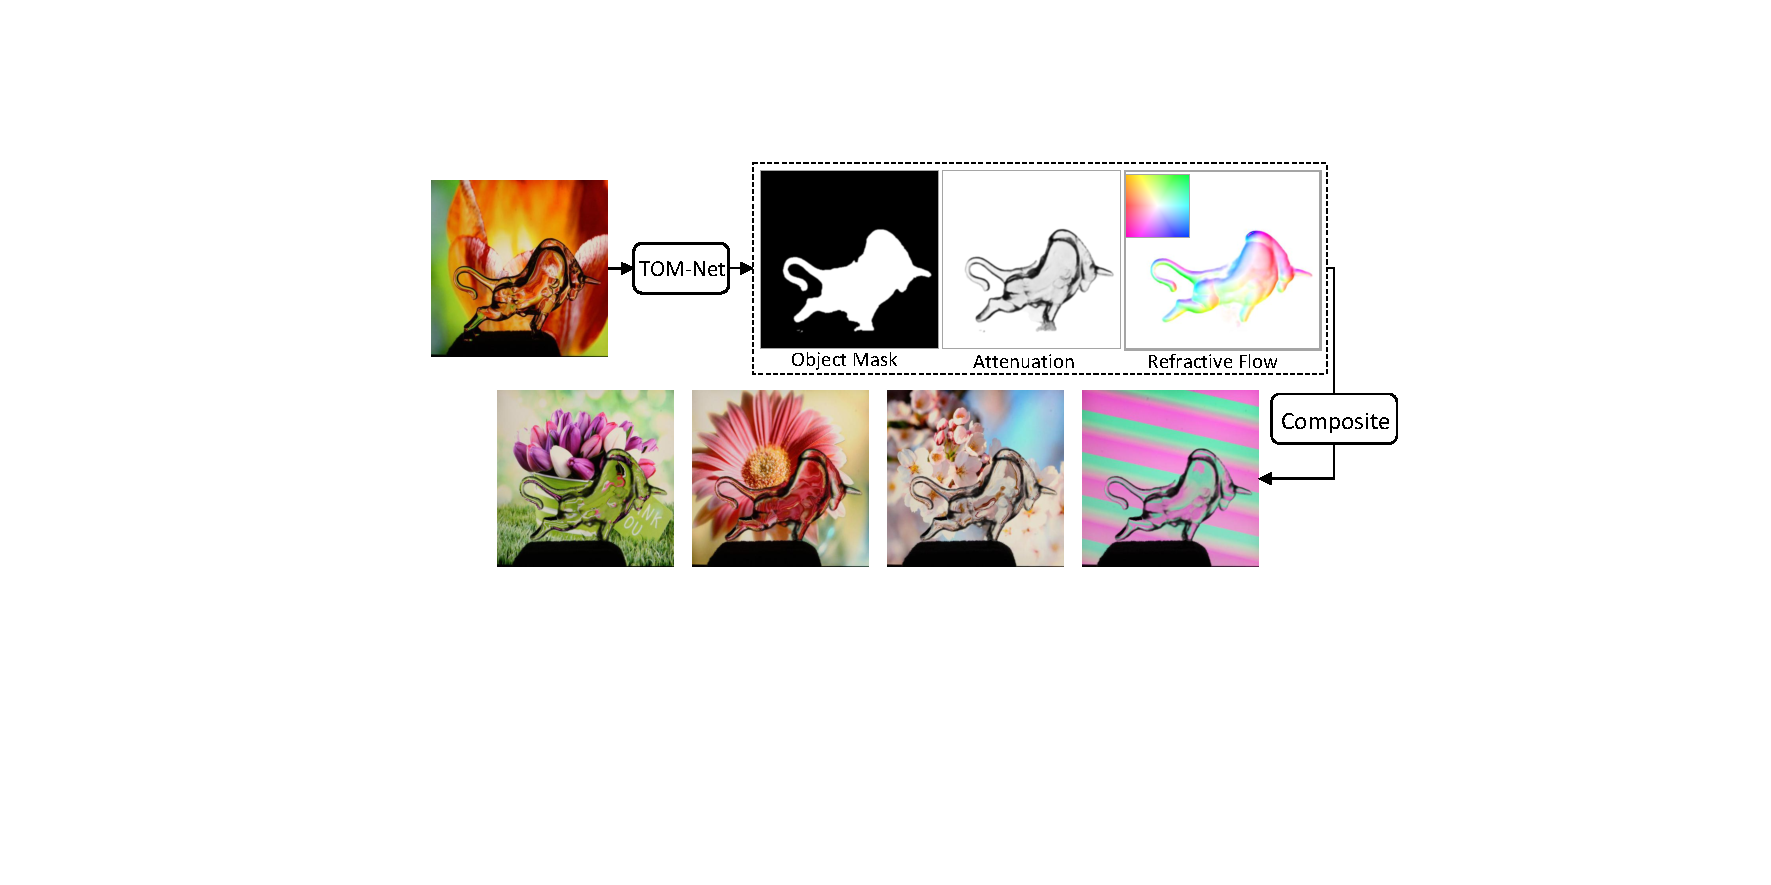
\includegraphics[width=0.8\linewidth]{images/network_intro_v3}
    \end{center}
    \vspace{-1em}
    \textbf{\color{blue}Motivations:}
    \begin{itemize}
        \item Existing alpha matting method cannot model the refractive effect of the transparent object.
    \begin{center}
        \vspace{-0.7em}
        \centering\includegraphics[width=0.25\linewidth]{images/{glass}.jpg}
        \centering\includegraphics[width=0.25\linewidth]{images/{alpha_matte}.png}
        \centering\includegraphics[width=0.25\linewidth]{images/{composite}.jpg}
        \\
        \vspace{-0.6em}
        \makebox[0.25\linewidth]{\scriptsize Photograph}
        \makebox[0.25\linewidth]{\scriptsize Alpha matte}
        \makebox[0.25\linewidth]{\scriptsize Composite}
    \end{center}
        \item \vspace{-0.8em}Existing matting approaches for transparent objects often require tedious capturing procedures and long processing time.
    \end{itemize}

    \vspace{0.2em}
    \textbf{\color{blue}Key Contributions:}
    \begin{itemize}
      \item A simple and efficient model for colorless transparent object matting. 
      \item A convolutional neural network, TOM-Net, for estimating an environment matte of a transparent object from a single image in a fast feed-forward pass. 
      \item A large-scale synthetic dataset and a real dataset as a benchmark for learning transparent object matting. 
    \end{itemize}  
}

%%%%%%%%%%%%%%%%%%%%%%%%%%%%%%%%%%%%%%%%%%%%%%%%%%%%%%%%%%%%%%%%%%%%%%%%%%%%%
\headerbox{\bf\color{blue} Problem Formulation}{name=formulation,column=1,row=0,span=1}{
    \textbf{\color{blue}Main idea:} We formulate transparent object matting as simultaneous estimation of an object mask, an attenuation mask and a refractive flow field.
    \begin{itemize}
        \item The original environment matting equation:
        \vspace{-0.5em} 
        \begin{equation}
            C = F + (1-\alpha)B + \sum_{i=1}^{m} R_i \mathcal{M}(\mathbf{T}_i, \mathbf{A}_i),
        \vspace{-0.2em} 
        \end{equation}
        where $F$, $B$ and $\alpha$ denote the ambient illumination, background color and opacity, respectively. $R_i$ is a factor describing the contribution of light emanating from the $i$-$th$ background image $\mathbf{T}_i$. $\mathcal{M}(\mathbf{T}_i, \mathbf{A}_i)$ denotes the average color of a rectangular region $\mathbf{A}_i$ on the background image $\mathbf{T}_i$.
        \vspace{0.2em}
    \item Considering a perfect transparent object and a single background image as the only light source:
        \vspace{-0.5em} 
        \begin{equation}
            C = (1-\alpha)B + R \mathcal{M}(\mathbf{T}, P),
        \vspace{-0.3em} 
        \end{equation}
        where $P$ is a point in the background $\mathbf{T}$.
    \item Assuming a colorless transparent object:
        \vspace{-0.5em} 
        \begin{equation}
            C = (1-\alpha)B + \rho \mathcal{M}(\mathbf{T}, P), \quad \rho \in [0, 1],
        \vspace{-0.3em} 
        \end{equation}
        where $R$ degenerates to a scalar attenuation $\rho$.
    \item Further introducing a binary foreground mask:
        \begin{equation}
            \label{eq:em_simplify3}
            C = (1 - m) B + m\rho \mathcal{M}(\mathbf{T}, P), \quad m \in\{0, 1\}.
        \end{equation}
    \item For each observed pixel $C$, we have to estimate 7 unknowns ($3$ for $B$, $2$ for $P$, $1$ for $m$ and $1$ for $\rho$).
    \end{itemize}
}

%%%%%%%%%%%%%%%%%%%%%%%%%%%%%%%%%%%%%%%%%%%%%%%%%%%%%%%%%%%%%%%%%%%%%%%%%%%%%
\headerbox{\bf\color{blue} Experiments \& Results}{name=results,column=2,row=0,span=2}{
    \textbf{\color{blue}Dataset:}

    \begin{minipage}{0.50\linewidth}
        \begin{itemize}
            \item We created a large-scale synthetic dataset for training and a real dataset for testing.
            \item Trained only on the synthetic dataset, TOM-Net can generalize well to real world objects, demonstrating its good transferability.
        \end{itemize}
        \begin{center}
            Statistics of the introduced datasets
        \resizebox{\linewidth}{!}{
        \begin{tabular}{c|*{6}{c}}
            \toprule
            Type & Glass & Glass \& Water & Lens & Complex & Total \\
            \midrule
            Synthetic Train & 52K & 26K & 20K & 80K & 178K\\
            Synthetic Val   & 250 & 250 & 200 & 200 & 900\\
            \midrule
            Real Test      & 470 & 103 & 61  & 242 & 876 \\
            \bottomrule
        \end{tabular}
        }
        \end{center}
    \end{minipage}
    \begin{minipage}{0.5\linewidth}
        \begin{center}
            Samples of synthetic data
            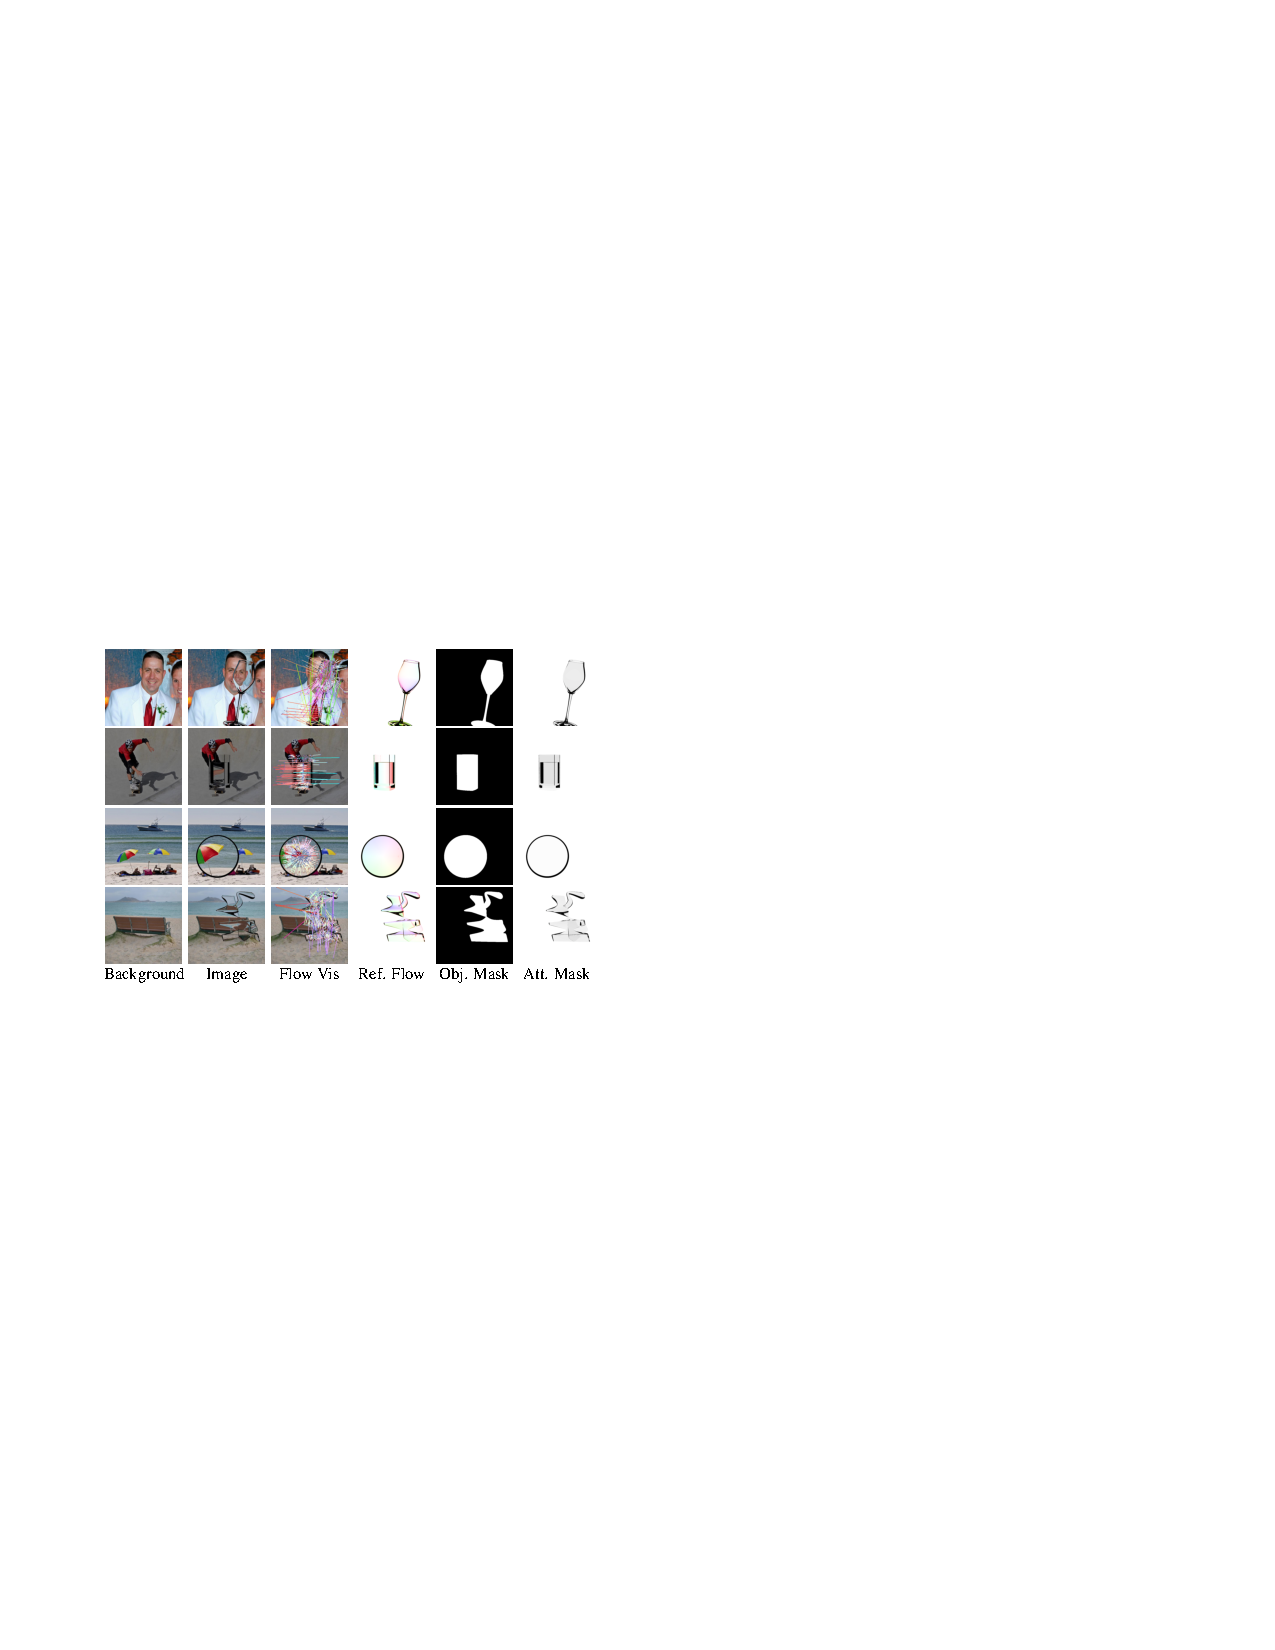
\includegraphics[width=\linewidth]{images/syn_data_sample}
        \end{center}
    \end{minipage}

    \textbf{\color{blue}Quantitative results on synthetic dataset:}

        \begin{minipage}{0.93\textwidth}
    \resizebox{\textwidth}{!}{
    \Huge
        \begin{tabular}{c|*{4}{c}|*{4}{c}|*{4}{c}|*{4}{c}|*{4}{c}}
        \toprule
        \multirow{2}{*}{} & \multicolumn{4}{c}{Glass} 
                               & \multicolumn{4}{c}{Glass with Water} 
                               & \multicolumn{4}{c}{Lens} 
                               & \multicolumn{4}{c}{Complex Shape}  
                               & \multicolumn{4}{c}{Average}  \\
                               & \cellcolor{red!25} F-EPE & \cellcolor{red!25}A-MSE & \cellcolor{red!25}I-MSE & \cellcolor{blue!25} M-IoU 
                               & \cellcolor{red!25} F-EPE & \cellcolor{red!25}A-MSE & \cellcolor{red!25}I-MSE & \cellcolor{blue!25} M-IoU 
                               & \cellcolor{red!25} F-EPE & \cellcolor{red!25}A-MSE & \cellcolor{red!25}I-MSE & \cellcolor{blue!25} M-IoU 
                               & \cellcolor{red!25} F-EPE & \cellcolor{red!25}A-MSE & \cellcolor{red!25}I-MSE & \cellcolor{blue!25} M-IoU 
                               & \cellcolor{red!25} F-EPE & \cellcolor{red!25}A-MSE & \cellcolor{red!25}I-MSE & \cellcolor{blue!25} M-IoU \\
        \midrule
        Background    & 3.6 / 30.3 & 1.33 & 0.48 & 0.12 & 6.4 / 53.2 & 1.54 & 0.68 & 0.12 & 10.3 / 39.2 & 1.94 & 1.57 & 0.24 & 6.8 / 56.8 & 2.50 & 0.85 & 0.11 & 6.8 / 44.9 & 1.83 & 0.90 & 0.15 \\
        CoarseNet     & 2.1 / 15.8 & 0.22 & 0.14 & 0.97 & 3.1 / 23.5 & 0.31 & 0.23 & 0.97 & 2.0 / 6.7   & 0.17 & 0.28 & 0.99 & 4.5 / 34.4 & 0.38 & 0.33 & 0.92 & 2.9 / 20.1 & 0.27 & 0.24 & 0.96 \\
        \midrule
        TOM-Net       & 1.9 / 14.7 & 0.21 & 0.14 & 0.97 & 2.9 / 21.8 & 0.30 & 0.22 & 0.97 & 1.9 / 6.6   & 0.15 & 0.29 & 0.99 & 4.1 / 31.5 & 0.37 & 0.32 & 0.92 & 2.7 / 18.6 & 0.26 & 0.24 & 0.96 \\
        \bottomrule
    \end{tabular}
    }
    \end{minipage}
    \hspace{-0.6em}
    \begin{minipage}{0.06\textwidth}
        \resizebox{\textwidth}{!}{
        \begin{tabular}{cc}
            \midrule
            MSE ($\cdot10^{-2}$) \\
            \cellcolor{red!25} $\downarrow$ better \\ 
            \cellcolor{blue!25} $\uparrow$ better\\
            \midrule
        \end{tabular}
        }
    \end{minipage}



    \vspace{0.5em}
    \textbf{\color{blue}Qualitative results on real dataset:}
    \begin{center}
        \vspace{-0.8em}
        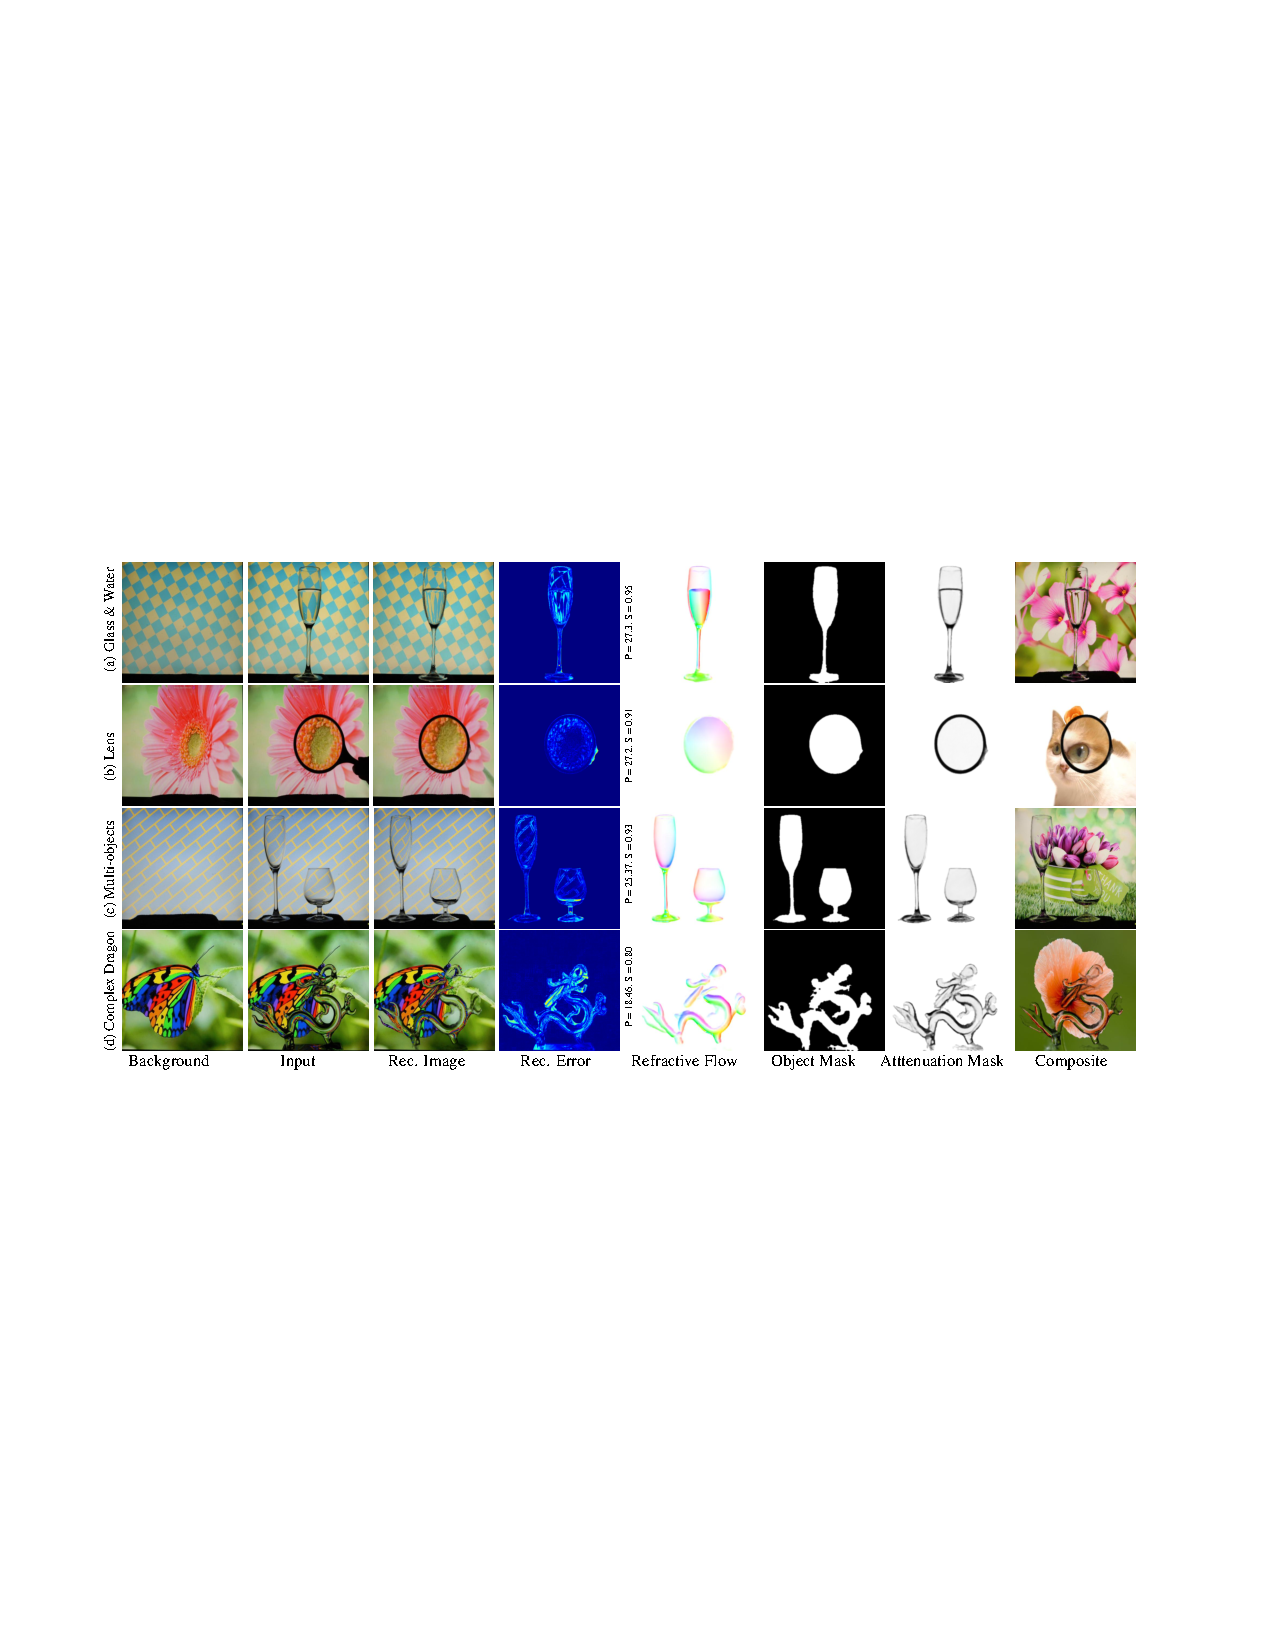
\includegraphics[width=0.92\linewidth]{images/real_qual.pdf}
        \vspace{-1em}
    \end{center}

    \vspace{0.5em}
    \begin{minipage}[t]{0.5\linewidth}
        \textbf{\color{blue}Visualization of the effectiveness of RefineNet:}

            \includegraphics[width=0.180\textwidth]{images/compare/{7_water5_0.90__6_tar}.jpg}
    \includegraphics[width=0.180\textwidth]{images/compare/{7_combine_flow}.jpg}
    \includegraphics[width=0.180\textwidth]{images/compare/{7_combine_r_flow}.jpg}
    \includegraphics[width=0.180\textwidth]{images/compare/{7_combine_rho}.jpg}
    \includegraphics[width=0.180\textwidth]{images/compare/{7_combine_r_rho}.jpg}
    \\
    \includegraphics[width=0.180\textwidth]{images/compare/{5_multi2_1.00__6_tar}.jpg}
    \includegraphics[width=0.180\textwidth]{images/compare/{5_combine_flow}.jpg}
    \includegraphics[width=0.180\textwidth]{images/compare/{5_combine_r_flow}.jpg}
    \includegraphics[width=0.180\textwidth]{images/compare/{5_combine_rho}.jpg}
    \includegraphics[width=0.180\textwidth]{images/compare/{5_combine_r_rho}.jpg}
    \vspace{-0.5em}
    \\
    \makebox[0.18\textwidth]{\footnotesize Input} 
    \makebox[0.18\textwidth]{\footnotesize Coarse Flow} 
    \makebox[0.18\textwidth]{\footnotesize Refined Flow} 
    \makebox[0.18\textwidth]{\footnotesize Coarse Att.} 
    \makebox[0.18\textwidth]{\footnotesize Refined Att.} 



    \end{minipage}
    \begin{minipage}[t]{0.5\linewidth}
        \textbf{\color{blue}Quantitative results on real dataset:}

            \resizebox{\textwidth}{!}{ 
    \huge
    \begin{tabular}{c|*{2}{c}|*{2}{c}|*{2}{c}|*{2}{c}|*{2}{c}}
        \toprule
        \multirow{2}{*}{} & \multicolumn{2}{c}{Glass} 
                          & \multicolumn{2}{c}{Glass \& Water} 
                          & \multicolumn{2}{c}{Lens} 
                          & \multicolumn{2}{c}{Complex} 
                          & \multicolumn{2}{c}{Avg} \\
        & PSNR & SSIM  & PSNR & SSIM & PSNR & SSIM & PSNR & SSIM & PSNR & SSIM \\
        \midrule
        Background    & 22.05 & 0.894 & 20.75 & 0.886 & 18.60 & 0.860 & 16.85 & 0.816 & 19.56 & 0.864 \\ 
        CoarseNet     & 25.09 & 0.921 & 23.53 & 0.911 & 21.13 & 0.895 & 17.89 & 0.835 & 21.91 & 0.891  \\ 
        TOM-Net        & 25.06 & 0.920 & 23.53 & 0.911 & 20.89 & 0.893 & 17.88 & 0.835 & 21.84 & 0.890 \\ 
        \bottomrule
    \end{tabular}
    }



        \hfill\begin{minipage}{0.46\linewidth}
            \begin{center}
            \textbf{Project Webpage}: \\
            \vspace{0.5em}\textbf{Code} \& \textbf{Dataset} \& \textbf{Model}
            \end{center}
        \end{minipage}
        \begin{minipage}{0.24\linewidth}
            \begin{center}
                
\includegraphics[width=\linewidth]{images/frame.png}
            \end{center}
        \end{minipage}
    \end{minipage}
}

%%%%%%%%%%%%%%%%%%%%%%%%%%%%%%%%%%%%%%%%%%%%%%%%%%%%%%%%%%%%%%%%%%%%%%%%%%%%%
\headerbox{\bf\color{blue} Method}{name=abstract,column=0,below=contribution,span=2}{
  TOM-Net comprises two parts, namely a multi-scale encoder-decoder network for producing a coarse prediction, and a residual network for refinement.
  \vspace{-0.2em}
  \begin{center}
   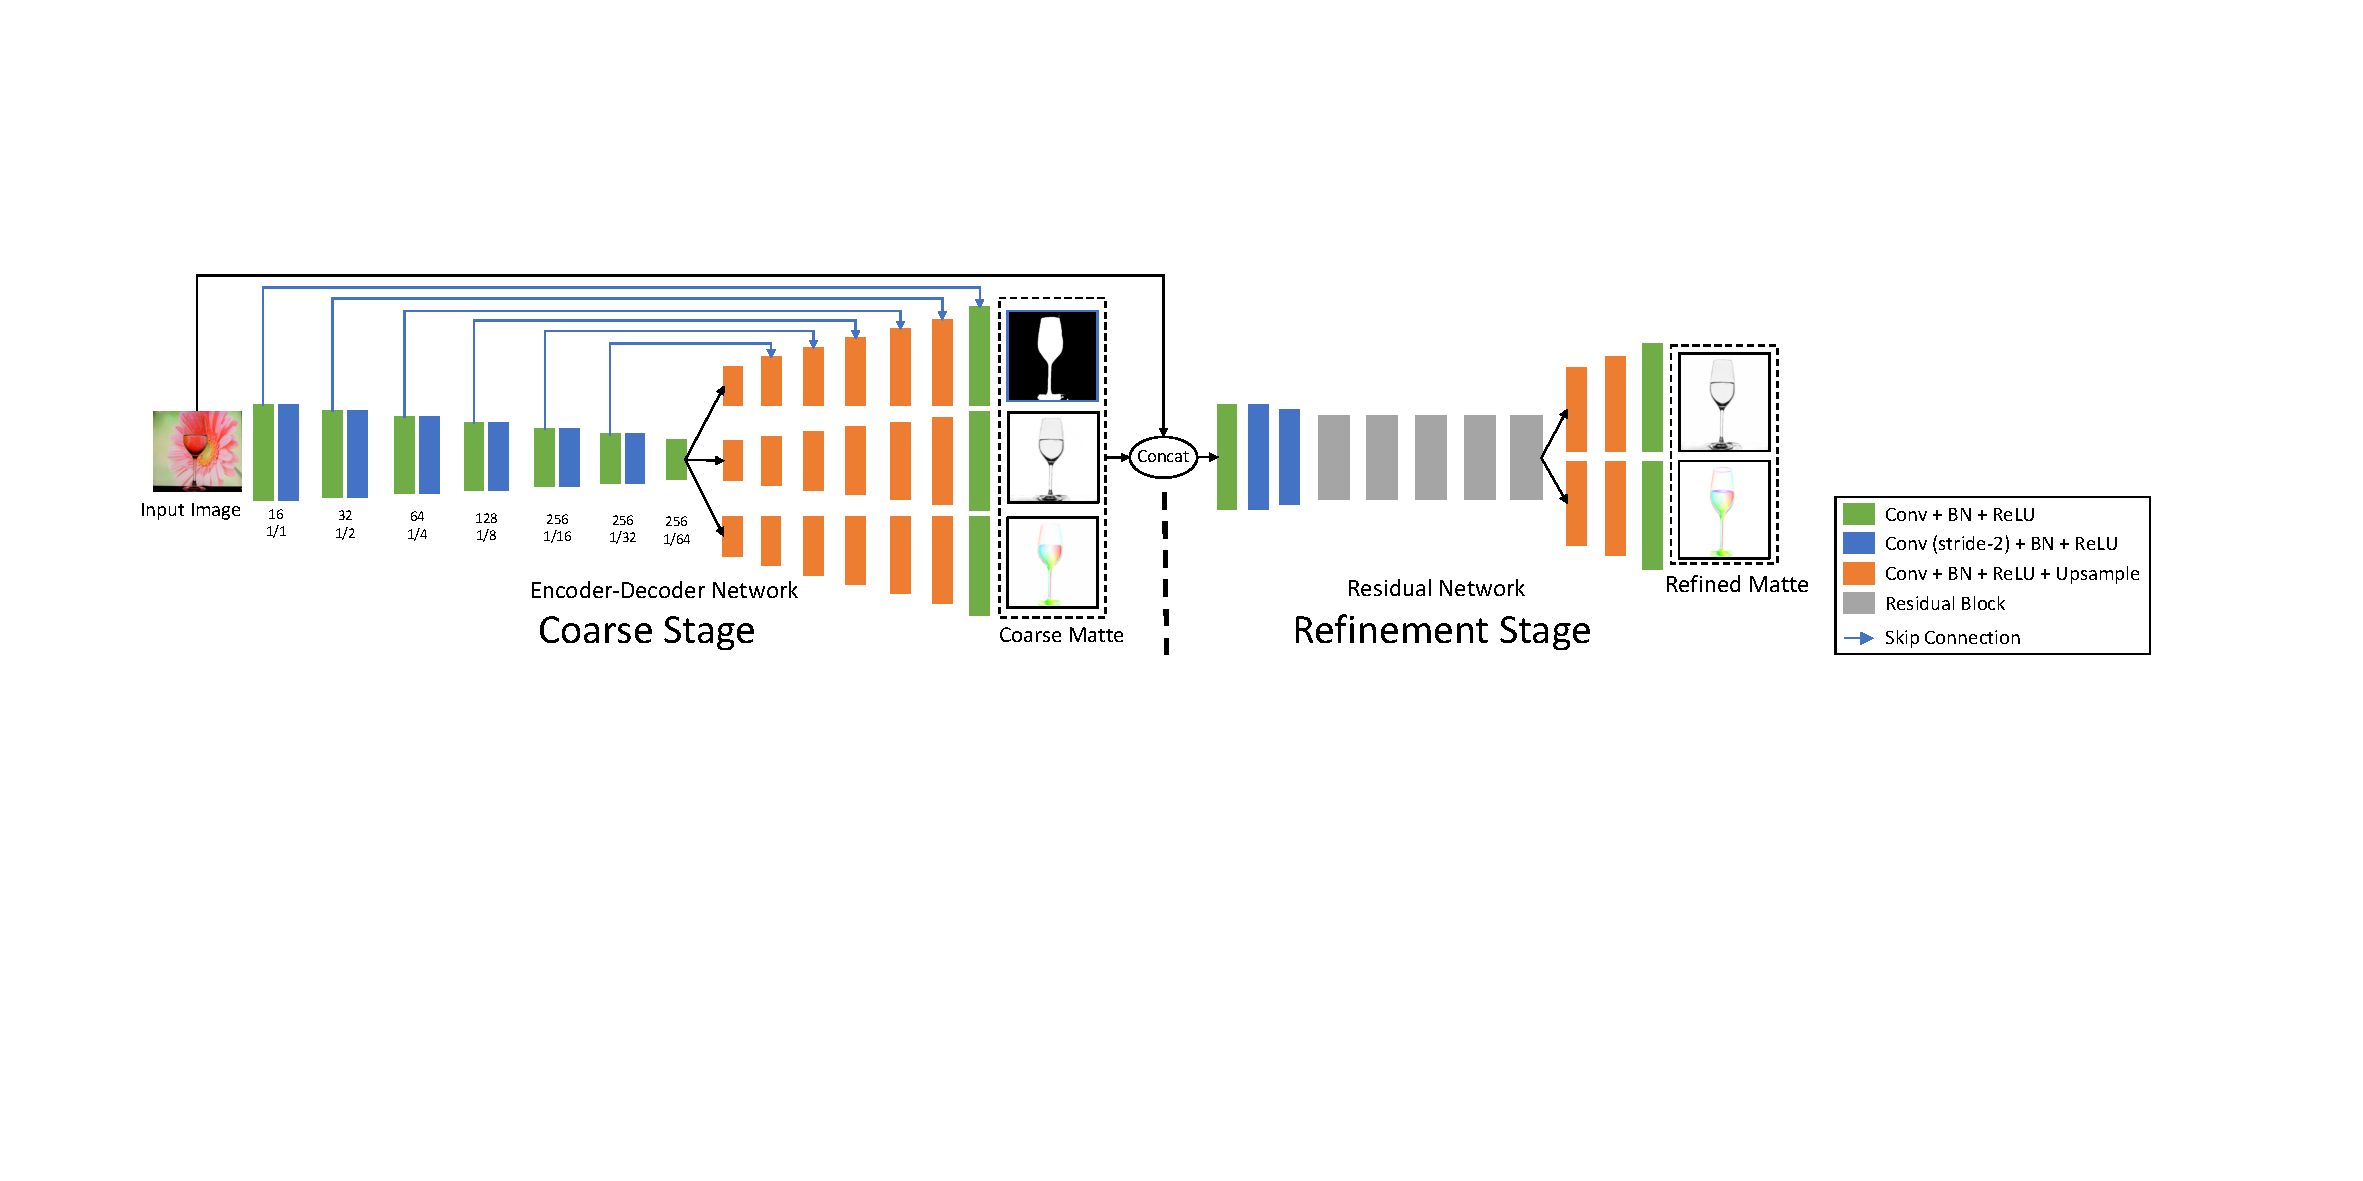
\includegraphics[width=0.9\textwidth]{images/framework_v3.pdf}
  \end{center}
  \vspace{-0.5em}
  \begin{minipage}[t]{0.48\linewidth}
 \textbf{\color{blue}Loss function for coase stage:}
    \vspace{-0.5em}
  \begin{align}
      \mathcal{L}^c = \alpha^c_{ms} \mathcal{L}_{ms} + \alpha^c_{ar} \mathcal{L}_{ar} + \alpha^c_{fr} \mathcal{L}_{fr} + \alpha^c_{ir} \mathcal{L}_{ir}
  \end{align}
  \begin{itemize}
    \vspace{-0.5em}
      \item $\mathcal{L}_{ms}$: Object mask segmentation loss (Cross entropy)
      \item $\mathcal{L}_{ar}$: Attenuation regression loss (MSE)
      \item $\mathcal{L}_{fr}$: Refractive flow regression loss (EPE)
      \item $\mathcal{L}_{ir}$: Image reconstruction loss (MSE)
      \item $\alpha^{c}_{\cdot}$: Weights for the loss terms
  \end{itemize}
  \end{minipage}
  \hfill
  \begin{minipage}[t]{0.48\linewidth}
    \textbf{\color{blue}Loss function for refinement stage:}
    \vspace{-0.5em}
    \begin{align}
        \mathcal{L}^r = \alpha^r_{ar} \mathcal{L}^r_{ar} + \alpha^r_{fr} \mathcal{L}^r_{fr} ,
    \end{align}
  \begin{itemize}
    \vspace{-0.5em}
      \item $\mathcal{L}^r_{ar}$: Refinement attenuation regression loss (MSE)
      \item $\mathcal{L}^r_{fr}$: Refinement refractive flow regression loss (EPE)
      \item $\alpha^{r}_{\cdot}$: Weights for the loss terms
  \end{itemize}
  \end{minipage}

}


\end{poster}
\end{document}
